\section{Introduction} 
\label{sec:intro}
Basic-block execution (BBE)

Discussion on single-threaded computing

Energy behavior or O3 and its shortcomings

Performance behavior of O3 and its benefits (speculation and dynamism)

Discussion of related papers that address above issues. items are: 
1) dynamism and speculation computing~\cite{dyn_specul},
2) multi-scalar
3) energy efficient computing (recent papers on this)

Contributions of this paper: 
1) coarse-grain execution model
2) energy driven design
3) performance aware design


\begin{figure}[h]
	\centering
	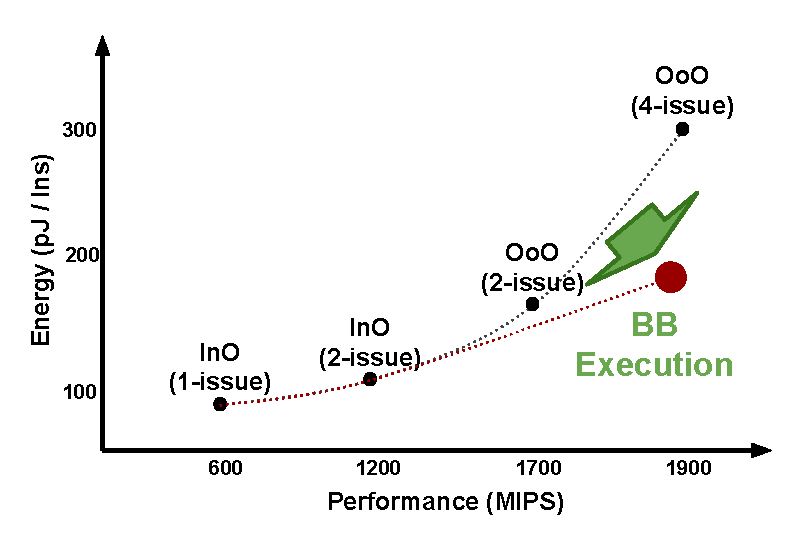
\includegraphics[width=1.0\columnwidth]{fig/energy_perf_insight.pdf} 
	\caption{Energy-Performance trend of recent micro-architectures}
	\label{fig:insight}
\end{figure}


% As described by~\cite{}, the exceptionally high
% performance of out-of-order (OoO) processors is fundamentally due to two key
% attributes: dynamism and speculation.  Lack of either feature can significantly
% impact its performance. 
% 
% The key sources of energy consumption in OoO processors is data-movement and XX
% (back this up).
% 
% Dynamism and speculation enable significant single-threaded performance benefits
% through effective latency hiding of unpredictable events such as cache miss and
% control mis-speculation.  Despite their performance advantages, dynamism and
% speculation cause a significant energy overhead for keeping track of instruction
% states and on-chip data movement; this energy overhead can be acceptable when,
% in fact, an unpredictable event stalls the execution flow; otherwise, a
% statically scheduled program can perform at least as well as a
% dynamically generated schedule.
% 
% The key contribution of this work is a scheduling model that combines static and
% dynamic scheduling with the gaol of reducing the processor energy overhead while
% maintaining near out-of-order (OoO) processor performance. Static scheduling provides
% fine-grain, optimal instruction-level scheduling while dynamic scheduling
% enables coarse grain, basicblock-level scheduling to dynamically hide
% unpredictable latencies.  In this model, each basicblock executes its
% instructions in-order while multiple basicblocks execute out of order with
% respect to one another.
